\documentclass[sokoban_generation_thesis.tex]{subfiles}

W literaturze była podjęta próba usprawnienia metody MCTS \cite{mcts_improve}. Zaprezentowano siedem usprawnień oryginalnej metody, jednak żadne z~nich nie poprawiło jej na~tyle, by~generowane poziomy zdaniem autora można było uznać za~zadowalająco skomplikowane.

\subsection{Wydajność czasowa} \label{subs:mcts_time}
\begin{figure}[h!]
	\centering
	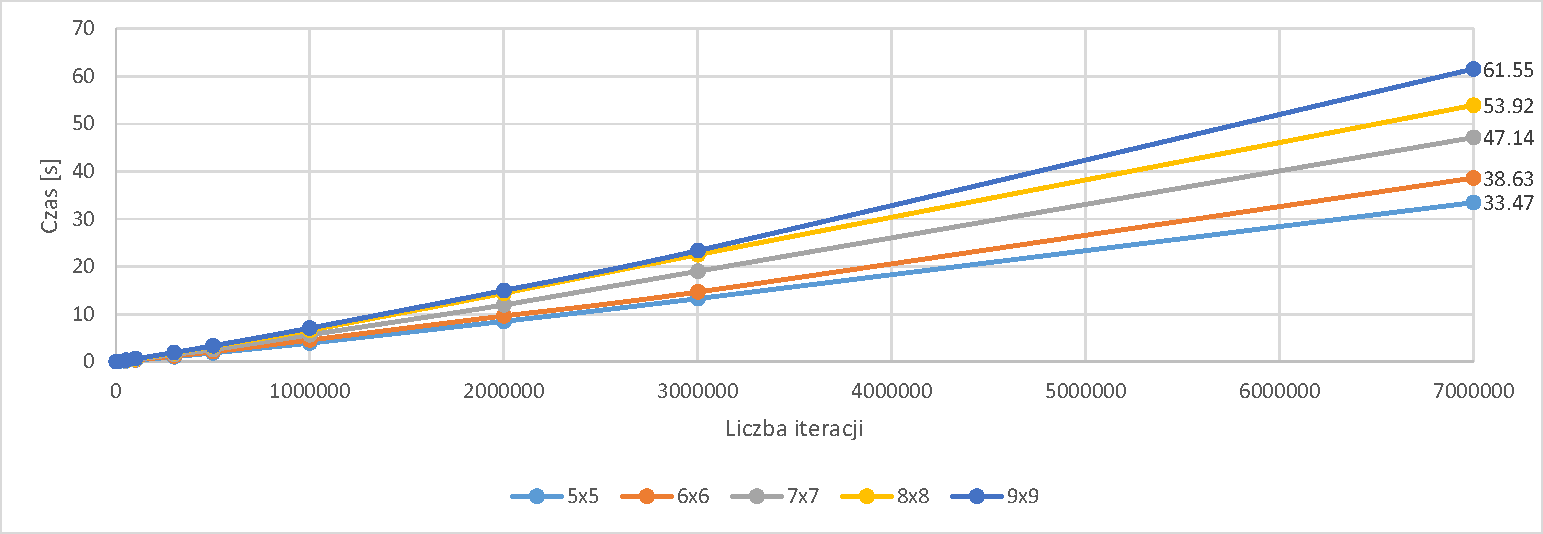
\includegraphics[width=0.9\textwidth]{mcts_czas_its}
	\caption{Zależność czasu od~liczby iteracji}
	\label{rys:mcts_czas_its}
\end{figure}

Wydajność czasowa metody jest najbardziej zależna od~czasu rozegrania pełnej zmodyfikowanej rozgrywki. W~prezentowanej implementacji liczba rozgrywek na~sekundę jest zależna od~rozmiaru planszy i~spada wraz z~ze~wzrostem liczby iteracji. Dla plansz o~boku krótszym niż sześć i~liczby iteracji mniejszych od~miliona, wykonywane jest aż~do trzystu tysięcy trywialnych rozgrywek na~sekundę. Ta~wydajność spada prawie dziesięciokrotnie dla większych plansz i~iteracji. W~celu przełożenia tej wydajności na~wartości czasowe, sporządzono wykres z~rys.~\ref{rys:mcts_czas_its}. Jak widać, dla siedmiu milionów iteracji metoda zakończy pracę po~trzydziestu sekundach dla planszy o~rozmiarze $5x5$, ale ta~sama praca dla planszy $9x9$ zostanie wykonana po~upływie minuty.

\subsection{Wydajność pamięciowa}
Zbadano ponadto zależność zużytej pamięci od~liczby iteracji i~maksymalnej liczby pudeł. Po~przeanalizowaniu wyników eksperymentu, wnioskuje się że~maksymalna liczba pudeł nie ma~istotnego wpływu na~zużytą pamięć. Za~to~wraz ze~wzrostem iteracji, liniowo zwiększa się zużyta pamięć. Czynnikiem który istotniej wpływa na~zużytą pamięć jest rozmiar planszy. Przeprowadzono eksperyment w~którym dla pięciu milionów iteracji zbadano zużycie pamięci w~zależności od~rozmiaru analizowanej planszy. Jak widać na~rys \ref{rys:mcts_ram_boardsize}, ta~zależność ma~charakter wykładniczy i~z~uwagi na~to, największy rozmiar planszy jaki udało się przeanalizować przy założonej liczbie iteracji to~$17$.

\begin{figure}[h!]
	\centering
	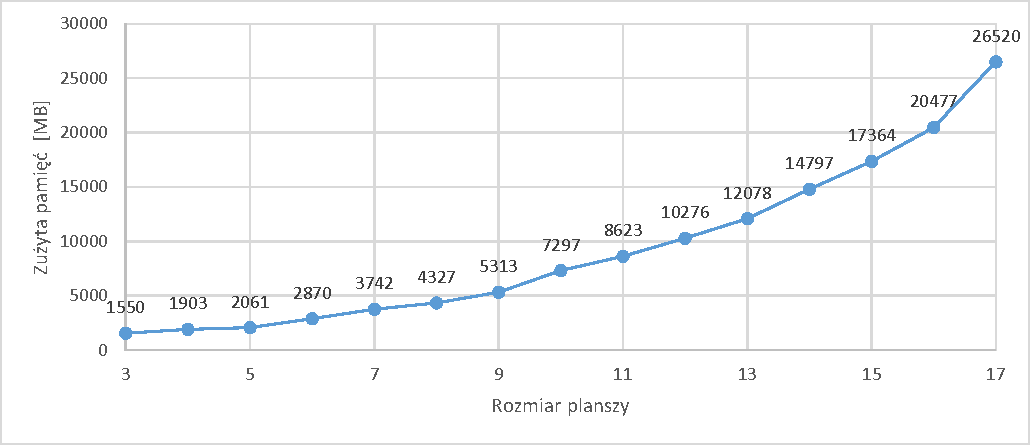
\includegraphics[width=0.9\textwidth]{mcts_ram_boardsize}
	\caption{Zależność zużytej pamięci od~rozmiaru planszy}
	\label{rys:mcts_ram_boardsize}
\end{figure}


\subsection{Wypłaty}
\begin{figure}[h!]
	\centering
	\begin{subfigure}[b]{0.3\textwidth}
		\centering
		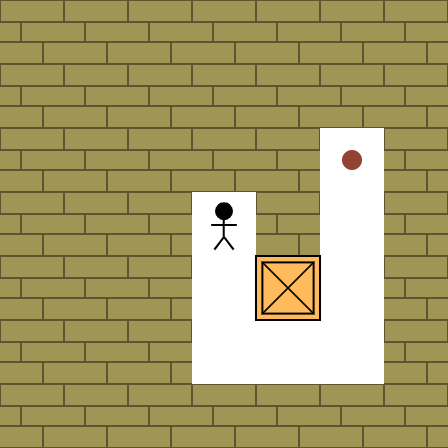
\includegraphics[width=0.8\textwidth]{board_mcts_step1}
		\caption{Iteracje: 100, wypłata: $0.22$}
	\end{subfigure}
	\begin{subfigure}[b]{0.33\textwidth}
		\centering
		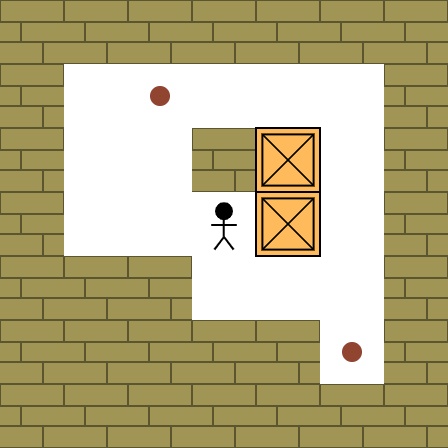
\includegraphics[width=0.7272\textwidth]{board_mcts_step2}
		\caption{Iteracje: $100000$, wypłata: $0.62$}
	\end{subfigure}
	\begin{subfigure}[b]{0.34\textwidth}
		\centering
		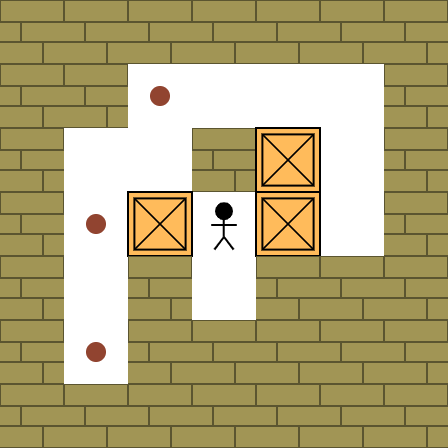
\includegraphics[width=0.70588\textwidth]{board_mcts_step3}
		\caption{Iteracje: $10000000$, wypłata: $1.1$}
	\end{subfigure}
	\caption{Rozwój generowanych plansz wraz ze~wzrostem iteracji}
	\label{rys:mcts_rozwoj}
\end{figure}

Wartość wypłaty za~wygenerowany poziom podczas wykonania metody MCTS powinna być tym wyższa, im~wygenerowana plansza jest bardziej skomplikowana, co~zostało opisane w~p.~\ref{subs:mcts_payoff}. Przykładowy rozwój generowanych plansz wraz z~wypłatami zaprezentowano na~rys.~\ref{rys:mcts_rozwoj}. Postanowiono zbadać, jak zmienia się najwyższa wypłata podczas kolejnych iteracji. Poznanie tej zależności pozwoliłoby na~odpowiednio wczesne przerywanie działania metody, w~zależności od~potrzeb. Jak widać na~rys.~\ref{rys:mcts_wyplaty_its}, wartość maksymalnej wypłaty jest istotnie różna dla różnych rozmiarów plansz.

\begin{figure}[h!]
	\centering
	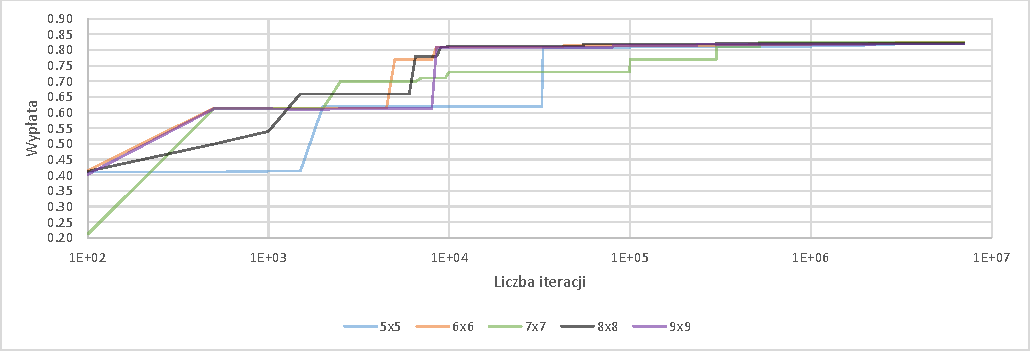
\includegraphics[width=0.9\textwidth]{mcts_wyplaty_its}
	\caption{Zależność maksymalnej wypłaty od~liczby iteracji}
	\label{rys:mcts_wyplaty_its}
\end{figure}

Autorzy metody MCTS podają za~jej zaletę fakt, iż~podczas jej działania niemal co~każdą iterację generowana jest pewna plansza w~wyniku losowej rozgrywki. W~celu zweryfikowania użyteczności sekwencji generowanych plansz, dokonano analizy średnich wypłat dla algorytmu działającego przez milion iteracji. Wyniki analiz zaprezentowano na~rys.~\ref{rys:mcts_sekwencja_wyplat}. Jak widać, niecałe $20\%$ generowanych plansz przekracza próg wypłaty $0.5$, a~jedynie $0.3\%$ z~nich jest ocenione na~więcej niż $1.1$. Prezentowany rozkład oznacza, że~jedynie wąska podgrupa z~generowanych plansz może być uznana za~wystarczająco skomplikowaną.


\begin{figure}[h!]
	\centering
	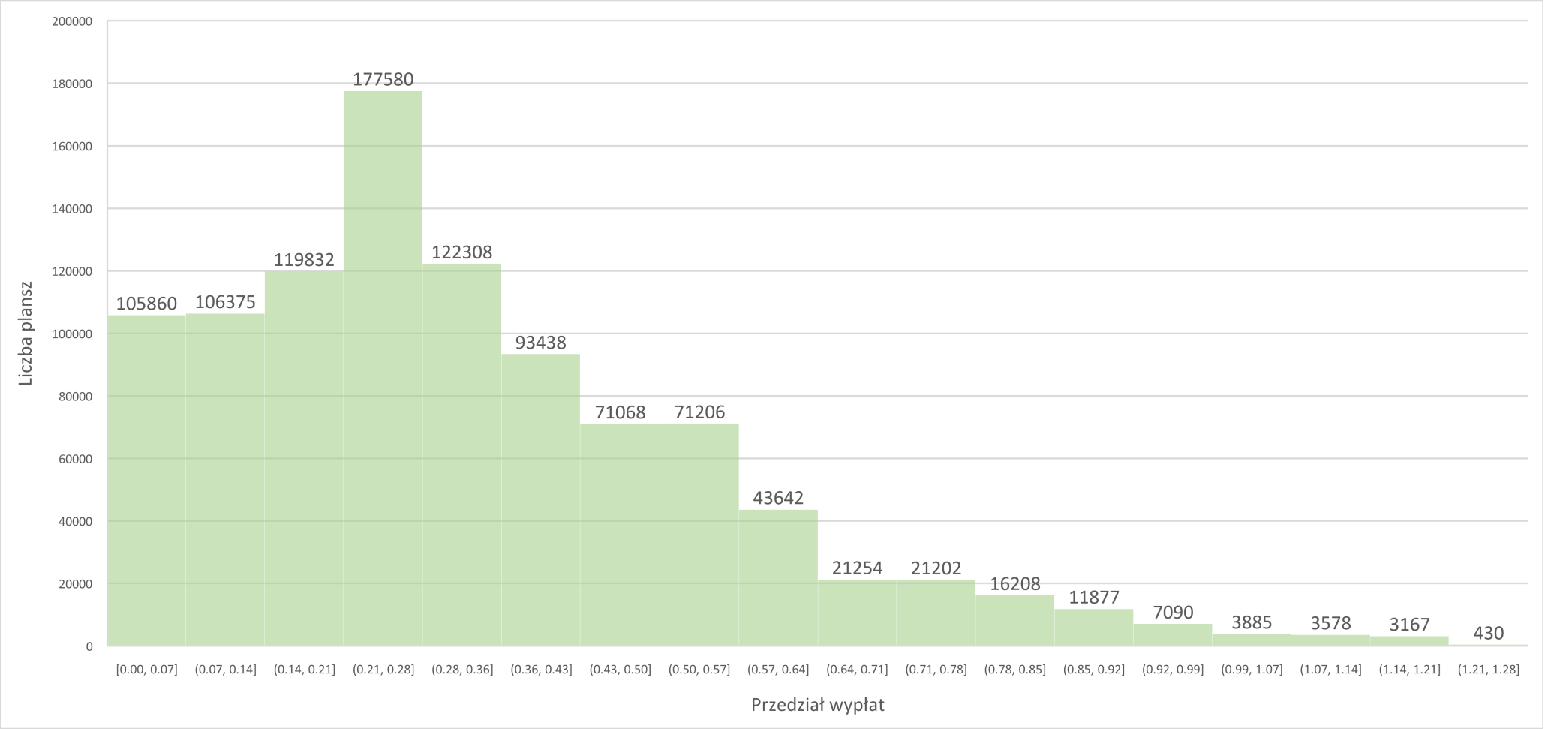
\includegraphics[width=0.9\textwidth]{mcts_sekwencja_wyplat}
	\caption{Rozkład wypłat dla generowanych plansz podczas miliona iteracji}
	\label{rys:mcts_sekwencja_wyplat}
\end{figure}

